\section{Background and Related Work}
\label{sec:background_related_work}

\subsection{Background}

\textbf{DMARC role in email communication.}
~\cref{fig:background} depicts a simplified overview of the \gls{DMARC} role in email communication.
Bob (sending domain) sends an email to Alice (receiving domain).
Alice queries Bob's \gls{DNS} server to retrieve \gls{DKIM}, \gls{SPF}, and \gls{DMARC} records to verify the email's authenticity and decide whether to deliver it.
When a \texttt{rua} address is present, Alice's email server is requested to report to Bob.
The reports provide insights into how Bob's domain is used and whether it is legitimate.
%The email communication sequence is as follows, where steps 3 and onwards are not part of the email sending process:
%1. Bob composes an email to Alice, where \gls{SMTP} message headers are set.
%2. Alice's email server (receiving \gls{MTA}) queries Bob's \gls{DNS} server (sender). The receiving \gls{MTA} retrieves the \gls{DKIM}, \gls{SPF}, and \gls{DMARC} rules from the TXT record and runs \gls{DKIM}, \gls{SPF}, and \gls{DMARC} verifications to decide whether to deliver the email to Alice's inbox (if positive verification) or not (if negative verification).
%3. After a period of time, Alice checks Bob's \gls{DMARC} \texttt{rua} to report \gls{DMARC} results. If Bob has specified sending \gls{DMARC} to external domains, then Alice queries those domains to confirm acceptance.
%4. With a confirmation, Alice's email server sends the report to the report processing service.
%5. The organization processes the \gls{DMARC} reports and provides them to Bob with insights. The insights help Bob to understand how his domain is used, the presence of an ongoing phishing campaign using its domain name, or whether there is a misconfiguration (with \gls{DKIM}, \gls{SPF}, or \gls{DMARC}) that is causing legitimate emails to be dropped before landing in the destination email inboxes.

\begin{figure}[tb]
\centering
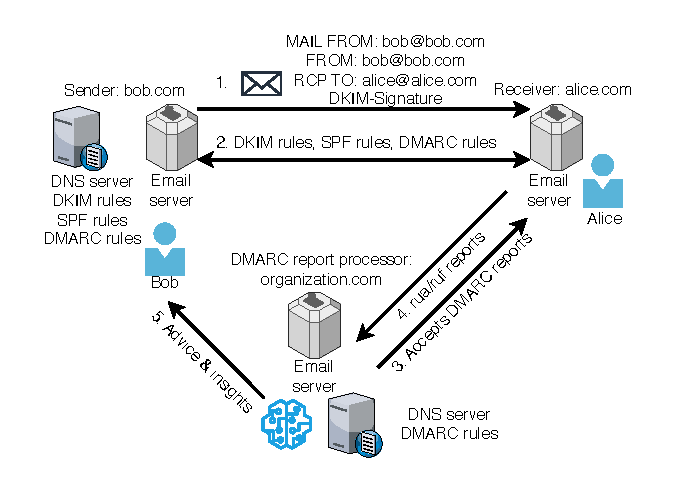
\includegraphics[width=.7\linewidth]{figures/dmarc-background.pdf}
\caption{Overview of DMARC role in email communication.}
\label{fig:background}
\vspace{-15px}
\end{figure}

\textbf{\acrfull{DKIM}.}
\acrshort{DKIM} is an email authentication and integrity verification method that employs public-key cryptography. Domain owners use \gls{DKIM} to digitally sign emails from their domain. During the \gls{SMTP} communication, the sender adds the \texttt{DKIM-Signature} header field with \gls{DKIM} relevant tags. For example, the signing domain (``d'' tag), a key selector (``s'' tag), and a signature (signed with the sender's private key, ``b'' tag).
The recipient's email server queries the sender's \gls{DNS} server for its TXT record (\eg \textit{<s>.\_domainkey.<d>.example.com}) to retrieve the public key, and then uses it to verify the received email signature. The verification results can be either \textit{pass}, \textit{permfail}, or \textit{tempfail}. Multiple signatures can be present in an email, and if at least one is valid, \gls{DKIM} evaluation succeeds.
% https://easydmarc.com/blog/what-are-dkim-tags/
% https://dmarcly.com/blog/how-to-implement-dmarc-dkim-spf-to-stop-email-spoofing-phishing-the-definitive-guide#what-is-dkim

\textbf{\acrfull{SPF}.}
\acrshort{SPF} allows a domain owner to specify a list of IP addresses that are authorized to send emails on behalf of their domain.
The domain owner configures the \gls{SPF} rules through the \gls{DNS} TXT record.
The recipient's mail server extracts the IP address and the domain name from ``MAIL FROM'' \textbf{or} ``HELO/EHLO FROM'' identify during the \gls{SMTP} communication.
\gls{SPF} verification is done through the \textbf{check\_host()} function~\cite{rfc7208}, which uses the identities and the sender's IP address from the \gls{SMTP} communication, and retrieves the \gls{SPF} rules to determine whether the sender's IP address belongs to the list of IP addresses configured.
The outcome can be either \textit{neutral}, \textit{pass}, \textit{fail}, \textit{softfail}, \textit{temperror}, or \textit{permerror}.
%The outcome of the verification can be \textit{none} (no conclusion about authorization), \textit{neutral} (treated as ``none''), \textit{pass}, \textit{fail}, \textit{softfail} (requires further investigation), \textit{temperror} (transient error during verification), or \textit{permerror} (incorrect \gls{SPF} records).
%The recipient's mail server can then decide to accept, reject, or mark the email as spam based on the verification result and their own anti-spoofing policies.
%\gls{DMARC} uses results of the \textbf{check\_host()} function based on ``MAIL FROM'' identity.
% https://www.rfc-editor.org/rfc/rfc7208#section-4 check\_host() function args

\textbf{\acrfull{DMARC}}
\gls{DMARC} data is published in the \gls{DNS} TXT records of the \textit{\_dmarc} subdomain (e.g., \textit{\_dmarc.example.com}). The record (\eg \texttt{v=DMARC1; p=reject; rua=mailto:rua@example.com}) always starts with the tag \texttt{v=DMARC1} followed by a list of tags separated by semicolons. The tags relevant to our study are:
\begin{itemize}
    \item[p] Policy for organizational domain. It tells the receiving mail server how to handle emails that fail \gls{DMARC} verification. The possible values are \texttt{none} (monitoring only), \texttt{quarantine}, and \texttt{reject} (block delivery).
    \item[sp] Similar to \texttt{p}, but for subdomains. If \texttt{sp} is not specified, the value of \texttt{p} tag is used. If the subdomain has its own \texttt{p} tag, then it takes precedence over the \texttt{sp} tag.
    \item[rua] Specify the email address(es) to which ``aggregate reports'' (see below) should be sent with ``mailto:address''. Multiple addresses can be specified.
    \item[ruf] Similar to \texttt{rua}, but for ``forensic reports'' (see below).
\end{itemize}

%\gls{DMARC} uses verification results from \gls{SPF} and \gls{DKIM} and also domain name alignment to determine the authenticity of an email.
%The \gls{SPF} domain name alignment occurs when the ``FROM'' domain name matches the ``MAIL FROM'' domain name of the received email.
%The \gls{DKIM} alignment occurs when the domain name present in the ``d'' tag matches the ``MAIL FROM'' domain name.
%\gls{DMARC} verification passes if \gls{SPF} check passes and the \gls{SPF} domain name is aligned \textbf{or} \gls{DKIM} check passes and the \gls{DKIM} domain name is aligned.

%\textbf{\gls{DMARC} reporting}
\gls{DMARC} sends two kinds of reports: \textbf{Aggregate} (in \texttt{rua} tag) and \textbf{Forensic} (in \texttt{ruf} tag)~\cite{rfc7489}. Aggregate reports provide a summary, in XML format, of \gls{DMARC}, \gls{SPF}, and \gls{DKIM} results (pass and fail), the sending IP address, \textit{RFC5322.From} address, etc.
The use of forensic reports is limited due to privacy concerns~\cite{hureau_stress_testing,_BSITR03182Email_}.
Reports help domain owners understand their domain's email usage, such as tracking policy effectiveness and spotting abuse or misconfigurations.
%The nature of forensic reports can lead to parties that receive such reports to have access to sensitive information, although previous work has shown that such reports are falling short of use~\cite{hureau_stress_testing}.\gls{DMARC} reports are often sent to another domain (\eg a specialized organization) for processing, as handling raw reports is complex~\cite{_DMARCReportsGoogle_}.

\subsection{Related work}
\gls{DMARC} adoption has been widely studied.
Durumeric \etal studied adoption of \gls{DMARC} in its early days. However, back then, the adoption was low even on popular domains~\cite{zakir2015}.
Hureau \etal~\cite{hureau_spoofed} carried out \gls{DNS} measurements using domain names from \glspl{gTLD}, \gls{CT} logs, and the tranco list, and used passive DNS data from SIE EU to study \gls{DMARC} preferences.
They showed the distribution of \gls{DMARC} policies and common mistakes in \gls{DMARC} records.% tags, and that popular domains are better configured with their \gls{DMARC} rules.
Maroofi's \etal study \gls{DMARC} adoption and subdomain spoofing~\cite{MaroofiEtAl_AdoptionEmailAntiSpoofing_2021}.
They used \glspl{gTLD}, \texttt{.se}, \texttt{.nu}, and samples of Rapid7 in their analysis, including a set of 32,042 unique high-profile domains (well-known companies, banks, and governments) from 139 countries.
In their modeled scenario, spoofed emails can reach the recipient's inbox via subdomains when the \gls{DMARC} policy is not strict enough.
In contrast, our paper focuses on the stringency of \gls{DMARC} policies across nearly all countries, surpassing prior work in the number of \glspl{ccTLD} covered by using a comprehensive \dataset. We go beyond and characterize government domains in isolation rather than grouped with domain names from different sectors.

The \gls{DMARC} reporting system had also been explored.
Hureau \etal tested the use of \gls{DMARC} reporting across different email service providers, focusing on the supported \gls{DMARC} features. They also tested the quality of reports that organizations or individuals receive~\cite{hureau_stress_testing}.
In another study, Hureau \etal showed the centralization of \gls{DMARC} report receivers~\cite{hureau_spoofed}. They documented the use of external destinations.
Ashiq \etal investigated the senders and receivers of \gls{DMARC} reports, showing that in some cases reports are not sent due to misconfigurations~\cite{ashiq2023}. Furthermore, their study revealed that 70\% of domains were configured with \gls{DMARC} to send reports to external domains.
Our paper provides a complementary perspective by examining the \gls{DMARC} reporting characteristics of domain names across \glspl{ccTLD} and demonstrating how these domain names depend on \gls{DMARC} report processors in foreign countries.
We analyze the use of \gls{DMARC} reporting in governmental domains and whether they follow their national security agencies' directives in this regard.
%Our \dataset provides a more comprehensive view of the \gls{DMARC} ecosystem from country-level perspective\rep.

